\section{Evaluation}
\label{sec:urltran:eval}
%
We now present the numerical evaluation of the different approaches presented in the previous sections.
Thereafter, we compare \URLTranSys to several recently proposed baselines.
We also report the model's training and inference times.
Finally, we analyze the robustness of the model \textit{adversarial test}  URLs.


\noindent\textbf{Setup:}
In our experiments, we set the hyperparameters for previously published models according to their settings in the original paper.
For evaluating \URLTranSysc, we vary the number of layers between $\{3, 6, 12\}$, vary the number of tokens per input URL sequence between $\{128, 256\}$.
We use both a byte-level and character-level BPE tokenizer with 1K- and 10K-sized vocabularies.
We randomly pick 15 hyperparameter combinations among these settings and present the results for these.
The Adam optimizer~\citep{kingma2014adam} is used in both pre-training and fine-tuning, with the triangular scheduler~\citep{smith2017cyclical} used for fine-tuning.
The hyperparameter settings for all models are provided in Section~\ref{sec:urltran:hyper}.
All training and inference experiments were conducted using PyTorch~\citep{pytorch} version 1.2 with NVIDIA Cuda 10.0 and Python 3.6.
The experiments were performed by extending the HuggingFace and Fairseq PyTorch implementations found on GitHub~\citep{huggingface,fairseq}.
Given the large class imbalance, accuracy is a poor metric of model performance.
To supplement accuracy, we evaluated all the models using the true positive rate (TPR) at low false positive rate (FPR) thresholds. 
We used the receiver operating characteristics (ROC) curve to compute this metric.


\noindent\textbf{Baselines:}
To evaluate the performance of our models, we compared them to two baseline phishing URL detection models: URLNet and Texception. URLNet~\citep{le2018malicious} is a CNN-based model which was recently proposed for the task of detecting URLs which identify malicious web sites. 
For comparison purposes, we trained and tested the URLNet model for the detection of phishing URLs.
Texception~\citep{tajaddodianfar2020texception} is another deep learning URL detection model for the task of identifying phishing URLs. 
Note that \citet{tajaddodianfar2020texception} compared Texception to a Logistic Regression-based model and found that Texception offered better performance.
Thus, we did not repeat that baseline experiment in this work.

\subsection{End-to-end Training}
%\noindent\textbf{\URLTranSysc.}
Transformers typically require large amounts of pre-training data (e.g., BERT~\citep{devlin2019bert} used a corpus of  $\approx$ 3.3 B tokens).
However, this data is derived from text articles, which are structured differently from URLs.
We trained the \URLTranSysc model based solely on the URL data found in our datasets to compare the results of finetuning using BERT (\URLTranSysb) and RoBERTa (\URLTranSysc) pretrained models to models pretrained only on in-domain URL data. 
The difference in dataset size and data domain make it important to understand the impact of different hyperparameters used when training transformers from scratch.
We compared runs across different hyperparameters on the basis of area under ROC (AUROC) and TPR@0.01\% FPR.
Figure~\ref{fig:urltran:pretrain_scratch} demonstrates that the training is not very sensitive to sequence length. 
Smaller byte-level vocabularies tend to be better overall, but at low FPR, the difference is not significant.
Finally, we found that the 3 layer model generalized the best.
We hypothesize that the better performance of the model with fewer layers is because of limited pre-training data.%\todo{pre-training vs pretraining consistent}
In the next few sections, we validate this hypothesis by evaluating fine-tuned model (\URLTranSysb, \URLTranSysr) that are tuned on a larger dataset.

\begin{figure}
\begin{subfigure}{0.48\linewidth}
	\centering
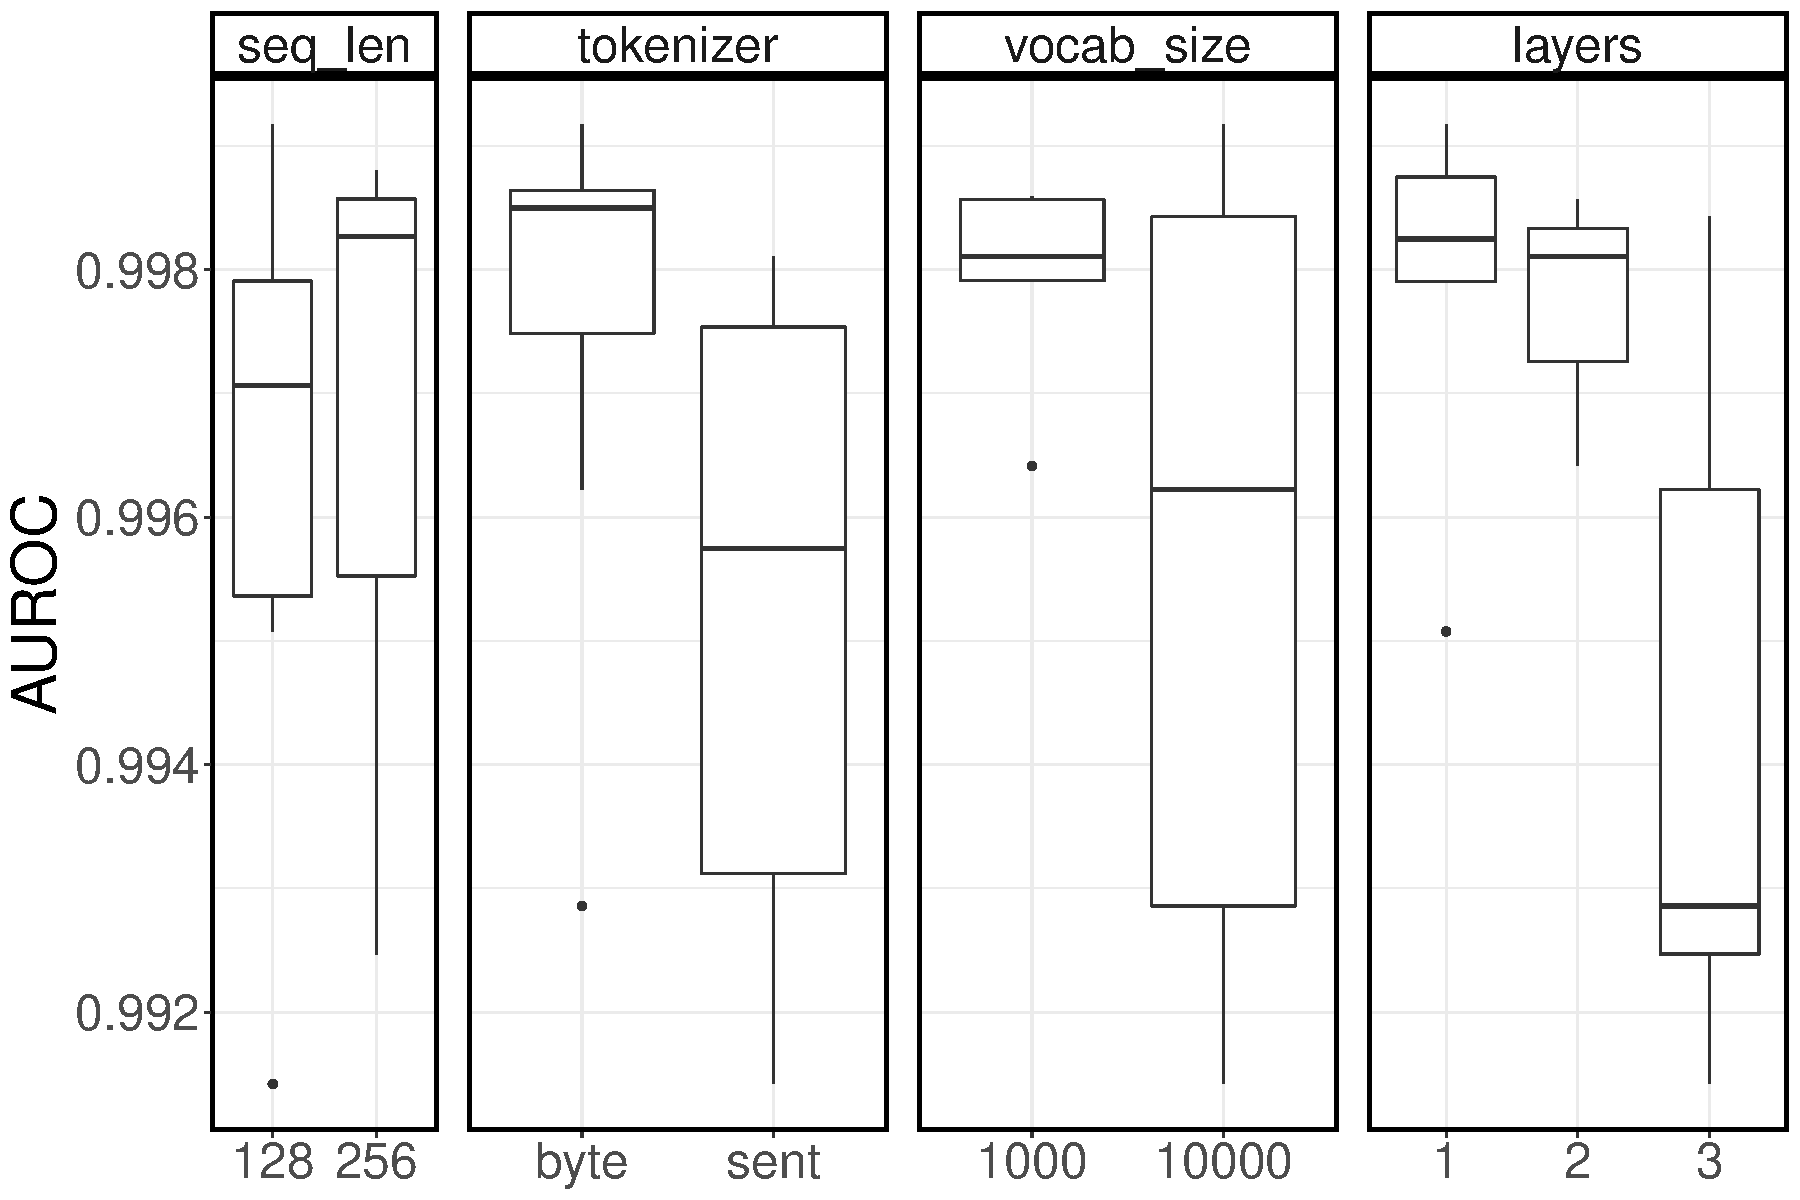
\includegraphics[width=0.95\linewidth]{urltran/figures/roc_hyperparams}
\caption{Area under ROC vs hyperparameters}
\label{fig:urltran:pretrain_scratch:roc}
\end{subfigure}
\begin{subfigure}{0.48\linewidth}
	\centering
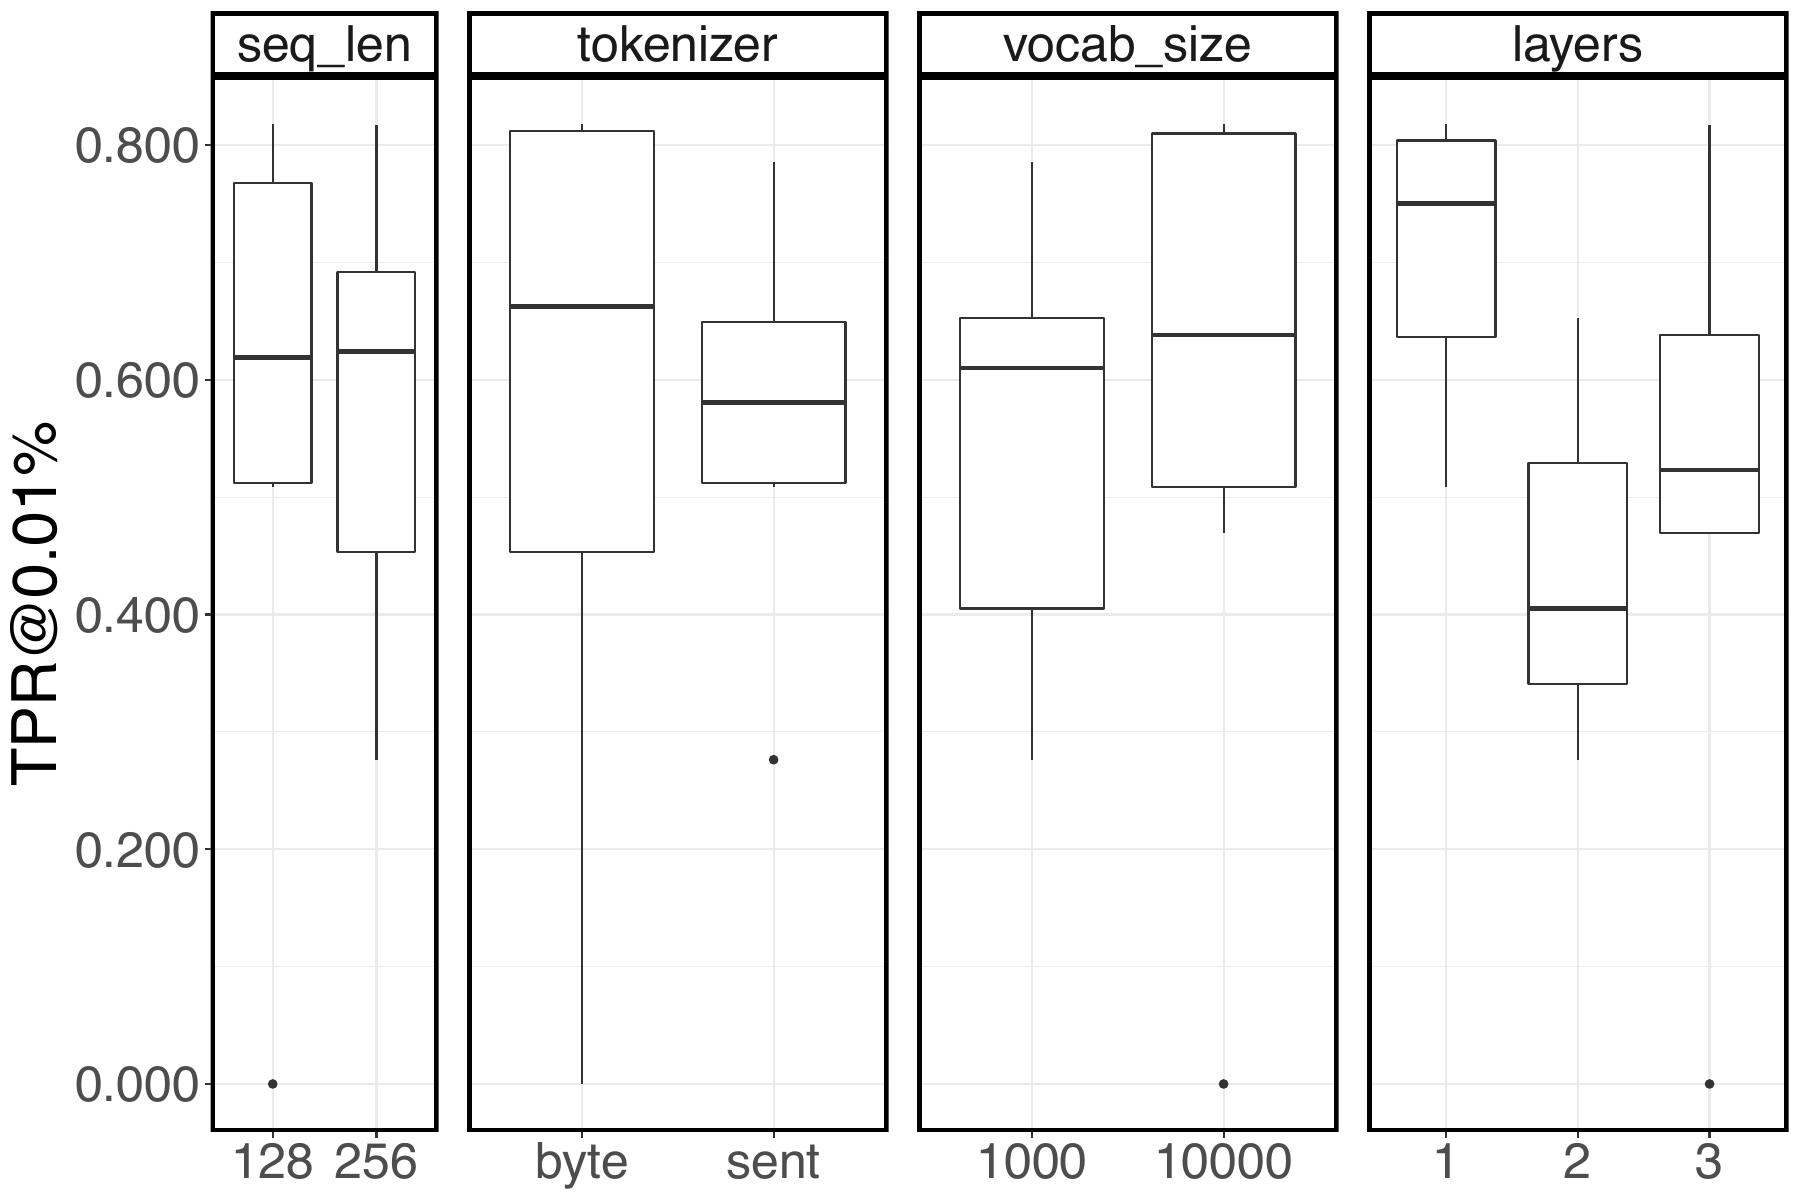
\includegraphics[width=0.95\linewidth]{urltran/figures/tpr_0.01_hyperparams}
\caption{TPR@FPR = 0.01\% vs hyperparmeters}
\label{fig:urltran:pretrain_scratch:tpr}
\end{subfigure}
\caption{Variance in quality of \URLTranSysc across different hyperparameter settings}\
\label{fig:urltran:pretrain_scratch}
\end{figure}


\subsection{Numerical Evaluation}


\begin{figure}
    \centering
	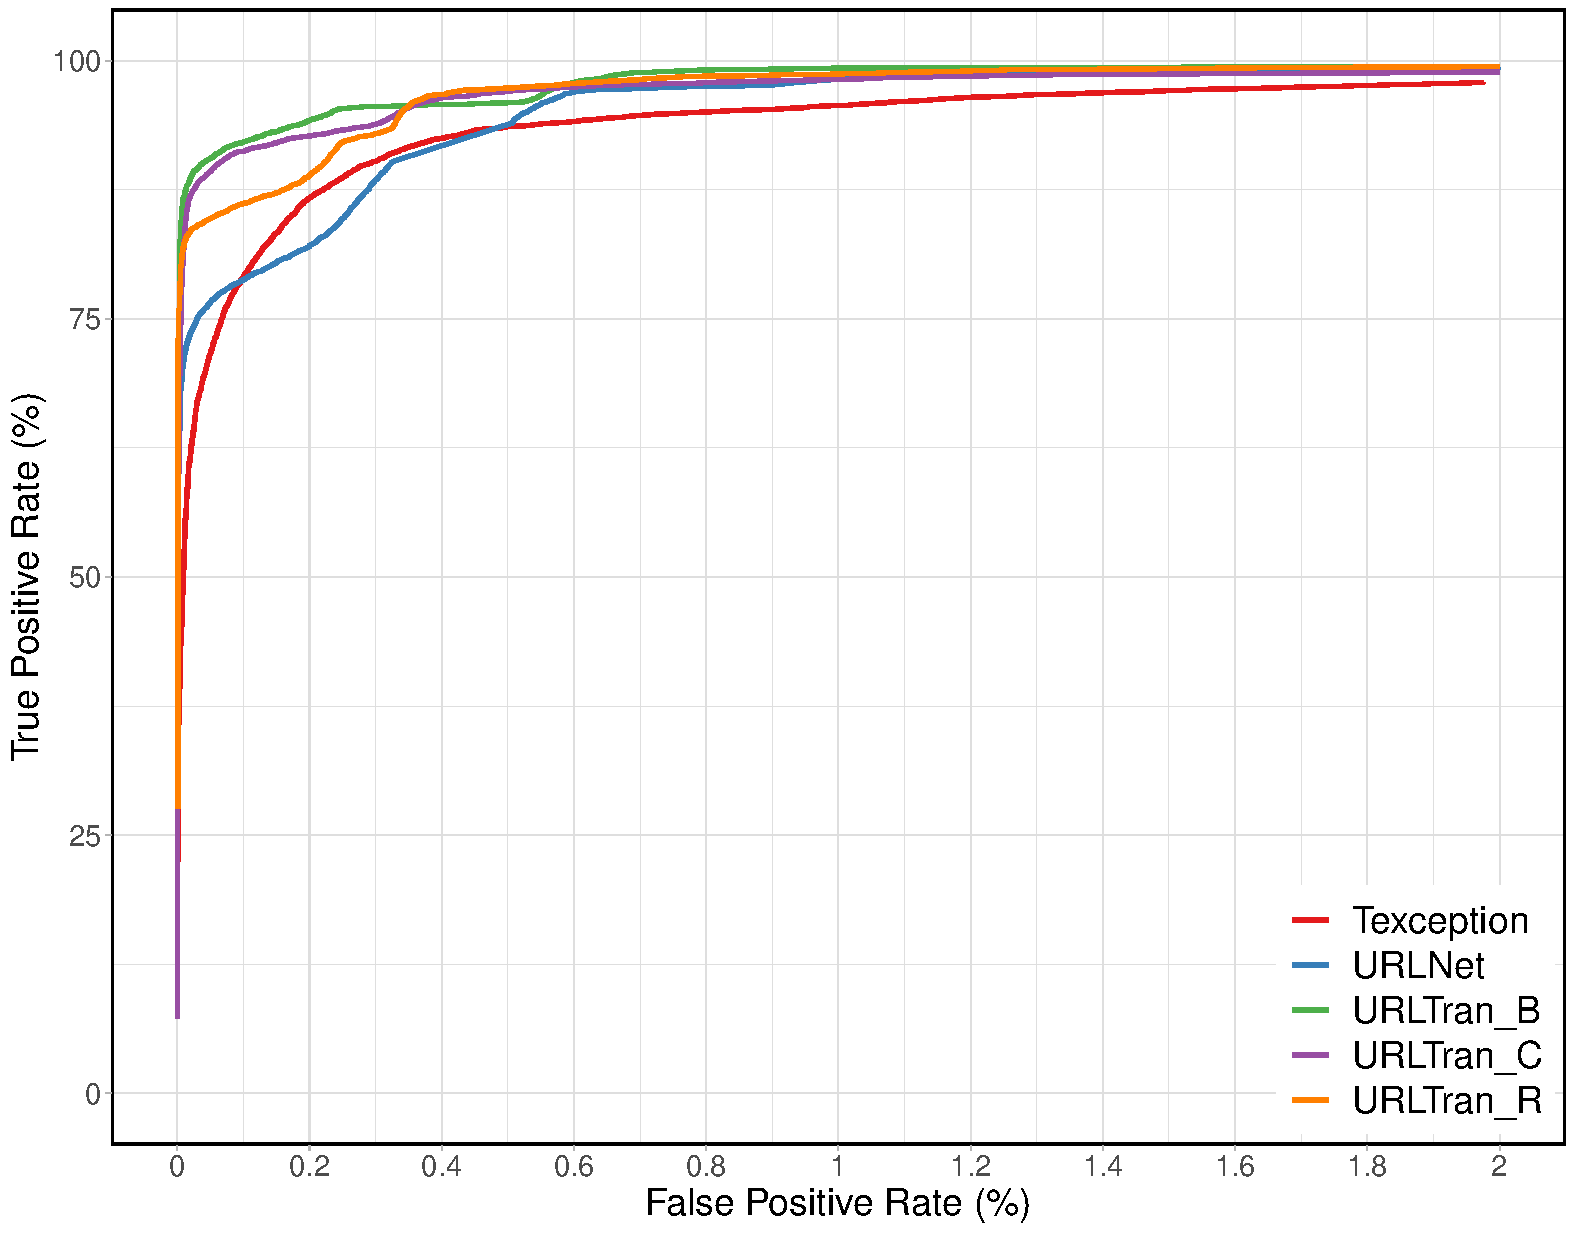
\includegraphics[width=0.7\linewidth]{urltran/figures/roc_0_02_R.pdf}
	\caption{Receiver operating characteristic curve indicating the performance of the \URLTranSys and several baseline models zoomed into a maximum of 2\% false positive rate.}
	\label{fig:urltran:transformer2}
\end{figure}

\begin{figure}
    \centering
	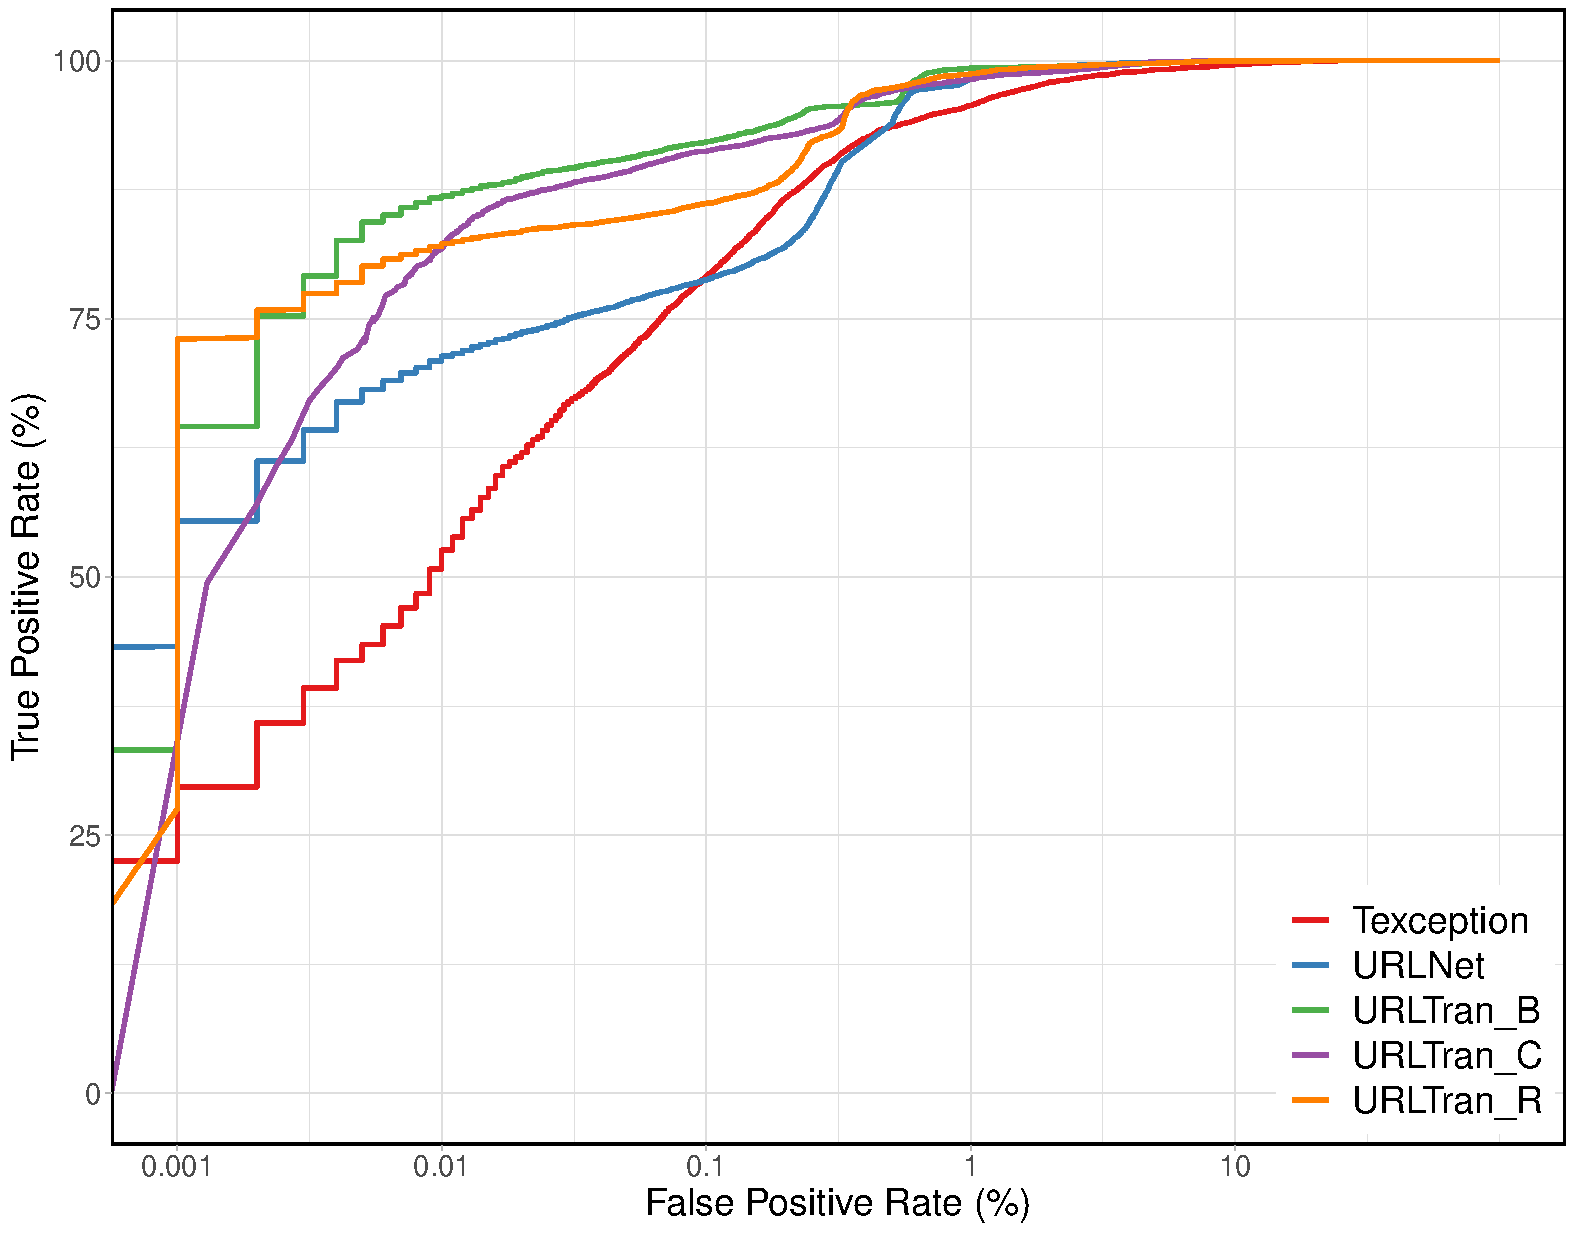
\includegraphics[width=0.7\linewidth]{urltran/figures/log_roc_R.pdf}
	\caption{Zoomed in receiver operating characteristic curve with a log x-axis.}
	\label{fig:urltran:log_transformer2}
\end{figure}



\noindent\textbf{Model Performance.}
We next analyzed the performance of the best parameters of all the proposed transformer variants.
To understand how these models compare at \textit{very low FPRs} where detection thresholds must be set to operate in a production environment, we first plotted the ROC curves on a linear x-axis zoomed into a 2\% maximum FPR in Figure~\ref{fig:urltran:transformer2}.
We also re-plot these ROC curves on a log x-axis in the semilog plot in Figure~\ref{fig:urltran:log_transformer2}.
These results indicate that all variants of \URLTranSys offer a significantly better
true positive rate over a wide range of extremely low FPRs. In particular, \URLTranSys matches or exceeds the TPR of URLNet for the FPR range of 0.001\% - 0.75\%.
The result is very important because phishing URL detection models must operate at very low FPRs (e.g., 0.01\%) in order to minimize the number of times the security service predicts that a benign URL is a phishing site (i.e., a false positive). In practice, the browser manufacturer selects the desired FPR and tries to develop new models which can increase the TPR for the selected FPR value.
Note that TPR@FPR is the standard metric commonly used both in production settings and in prior art such as Texception and URLNet.
In addition to the ROC curve analysis, we also summarize a number of key performance metrics in Table~\ref{tab:urltran:model-perf}, where `F1' is the F1 score, and `AUC' is the area under the model's ROC curve.
The proposed \URLTranSys model outperforms both Texception and URLNet for all of these metrics.
In particular, we note that  at an FPR
of 0.01\%, \URLTranSysb has a
TPR of 86.80\% compared to 71.20\% for URLNet and 52.15\% for Texception.

\begin{table}[ht]
\begin{center}
\resizebox{\linewidth}{!}{
\begin{tabular}{ccccccc}
\toprule
Model & Accuracy (\%) & Precision (\%) & Recall (\%) & TPR@FPR=0.01\% & F1 & AUC \\
\midrule
Texception & 99.6594 & 99.7562 & 99.6594 & 52.1505 & 0.9969 & 0.9977 \\
URLNet & 99.4512 & 99.7157 & 99.4512 & 71.1965 & 0.9954 & 0.9988 \\
\URLTranSysc & 99.5983 & 99.7615 & 99.5983 & 81.8577 & 0.9965 & 0.9992 \\
\URLTranSysr & 99.6384 & 99.7688 & 99.6384 & 82.0636 & 0.9968 & 0.9992 \\
\URLTranSysb & 99.6721 & 99.7845 & 99.6721 & 86.7994 & 0.9971 & 0.9993 \\
\bottomrule
\end{tabular}
}
\end{center}
\caption {Comparison of different performance metrics for \URLTranSys and the two baseline models.}
\label{tab:urltran:model-perf}
\end{table}


%\input{error}

\noindent\textbf{Training and Inference Times.}
The total time required to train the best \URLTranSysb model was 4:57:11 on an NVIDIA V100. Inference
required 0:10::44 to complete for an average of 0.36096 milliseconds per sample.


\begin{figure}
    \centering
	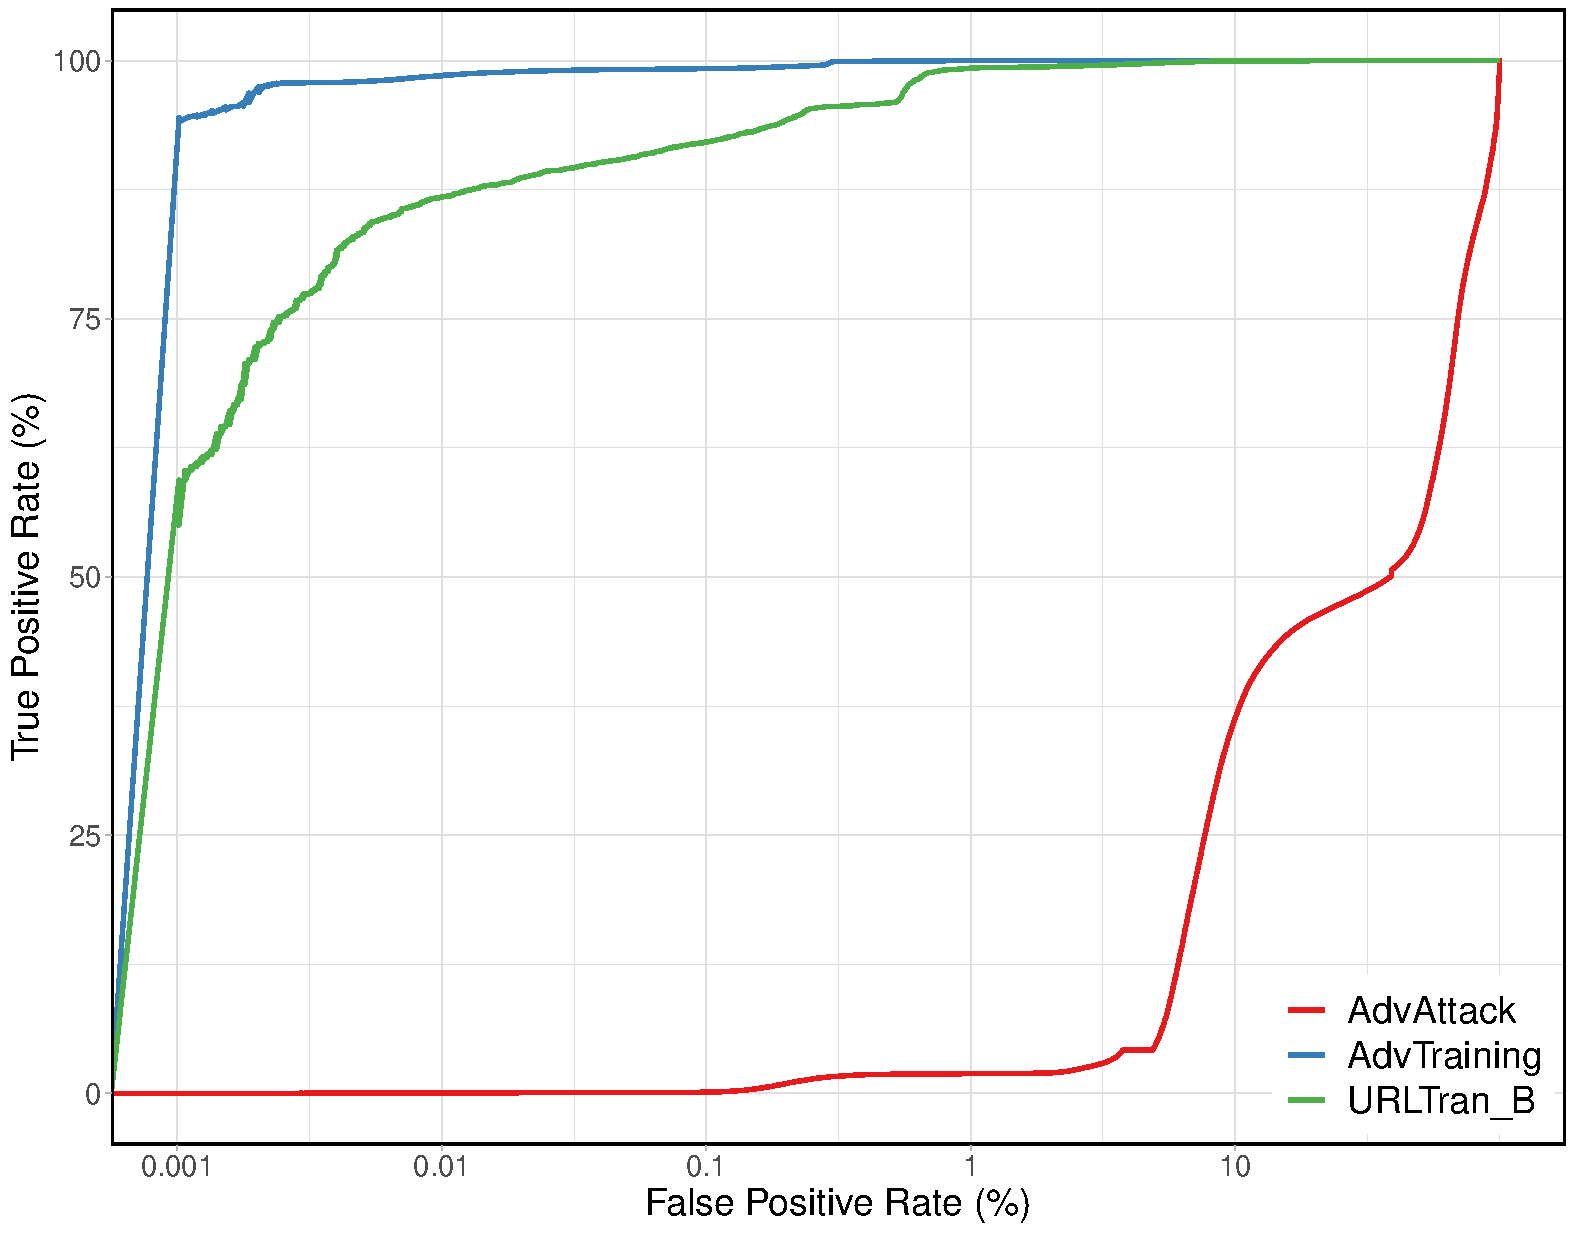
\includegraphics[width=0.7\linewidth]{urltran/figures/log_roc_adv_R}
	\caption{ROC curve for \URLTranSysb when under adversarial attack, and adversarial robustness after augmented training}
	\label{fig:urltran:adversarial_roc}
\end{figure} 

\subsection{Adversarial Evaluation.}
To understand \URLTranSys's robustness to adversarial attacks, we first compared the low FPR regions of the ROC curve of the unprotected model tested with the original test set to the
test set which includes adversarial samples (AdvAttack) generated through the methods described in Section~\ref{sec:urltran:adv_attack} (Figure~\ref{fig:urltran:adversarial_roc}).
There is a significant drop in performance of \URLTranSysb when attacked with adversarial URLs.
As discussed previously (Section~\ref{sec:urltran:adv_attack}, \textit{adversarial testing} provides a mechanism to ensure that models can be made robust to attacks that follow known threat models.
We test this hypothesis by considering the scenario where attack strategies are incorporated into the training data (AdvTraining).
\todo{Another place where covariate shift can be referenced.}
On the addition of adversarial attack patterns to the training, the model is able to  the adapt to novel attacks, and even exceeded the performance of the non-adversarially trained version of \URLTranSys.
These results demonstrate that  creating adversarial can help models such as \URLTranSys adapt to unseen attacks.
Further, as new attack strategies are recognized (e.g., alternative homoglyph), a robust version of \URLTranSys can be trained to recognize similar patterns in unseen test data.

\section{Hyperparameter Settings}
\label{sec:urltran:hyper}
For replicability, this sectino provides the hyperparameter settings for the three variants of the proposed \URLTranSys model as well as those for two baseline models.
Tables~\ref{tab:urltran:URLNetParams} and~\ref{tab:urltran:TexParams} list the hyperparameters for the URLNet and Texception models that we use
as baselines in our study. The hyperparameter settings for the best performing \URLTranSysb model are provided in Table~\ref{tab:urltran:TransParamsBert}.
In addition, the best hyperparameter settings for the \URLTranSysr and \URLTranSysc are given in Tables~\ref{tab:urltran:TransParamsRoberta} and~\ref{tab:urltran:TransParamsCustVoc},
respectively.

\begin{table}
\centering
\footnotesize
\begin{tabular}{lc}
\toprule
Parameter & Value \\
\midrule
max\_len\_words & 200 \\
max\_len\_chars & 1000 \\
max\_len\_subwords & 20 \\
min\_word\_freq & 1 \\
dev\_pct & 0.001 \\
delimit\_mode & 1 \\
emb\_dim & 32 \\
filter\_sizes & {[}3,4,5,6{]} \\
default\_emb\_mode & char + wordCNN \\
nb\_epochs & 5 \\
train\_batch\_size & 128 \\
train\_l2\_reg\_lambda & 0.0 \\
train\_lr & 0.001 \\
\bottomrule
\end{tabular}
\caption{Hyperparameters used for URLNet.}
\label{tab:urltran:URLNetParams}
\end{table}


\begin{table}
\centering
\footnotesize
\begin{tabular}{clc}
\toprule
\multicolumn{2}{c}{Parameter} & Value\\
\midrule
\multirow{5}{*}{
\vtop{\hbox{\strut Characters}\hbox{\strut Branch}}
} & embedding dimension & 32 \\
 & number of blocks & 1\\
 & block filters & {[}2,3,4,5{]}\\
 & Adaptive MaxPool output & 32,32\\
 & maximum characters & 1000\\
\midrule
\multirow{5}{*}{
 \vtop{\hbox{\strut Words}\hbox{\strut Branch}}
} & embedding dimension & 32\\
 & number of blocks & 1\\
 & block filters & {[}1,3,5{]}\\
 & Adaptive MaxPool output & 32,16\\
 & maximum words & 50\\
\midrule
\multirow{6}{*}{
\vtop{\hbox{\strut FastText}\hbox{\strut Model}}
} & minimum words to include & 50\\
 & vocabulary size & 120000\\
 & window size & 7\\
 & n-grams & 2-6\\
 & embedding dimension & 32\\
 & epochs trained & 30\\
\bottomrule
\end{tabular}
\caption{Hyperparameters used for Texception.}
\label{tab:urltran:TexParams}
\end{table}

\begin{table}
\centering
\footnotesize
\begin{tabular}{lc}
\toprule
Parameter & Value \\
\midrule
  attention probs dropout prob & 0.1 \\
  hidden act & gelu \\
  hidden dropout prob & 0.1 \\
  hidden size & 768 \\
  initializer range & 0.02 \\
  intermediate size & 3072 \\
  layer norm eps & 1e-12 \\
  max position embeddings & 512 \\
  num attention heads & 12 \\
  num hidden layers & 12 \\
  type vocab size & 2 \\
  vocab size & 30522 \\
  bert model & bert-base-uncased \\
  max seq length & 128 \\
  train batch size & 32 \\
  learning rate & 2e-5 \\
  num train epochs & 10 \\
  \bottomrule
\end{tabular}
\caption{Hyperparameters  used for training the proposed Huggingface-based \URLTranSysb model.}
\label{tab:urltran:TransParamsBert}
\end{table}

\begin{table}
\centering
\footnotesize
\begin{tabular}{lc}
\toprule
Parameter & Value \\
\midrule
Number of Layers & 12 \\
Hidden size & 768 \\
FFN inner hidden size & 3072 \\
Attention heads & 12 \\
Attention head size & 64 \\
Dropout & 0.1 \\
Attention Dropout & 0.1 \\
Warmup Steps & 508 \\
Peak Learning Rate & 1e-4 \\
Batch Size & 2k \\
Max Epochs & 10 \\
Learning Rate Decay & Linear \\
Adam $\epsilon$ & 1e-6 \\
Adam $\beta_1$ & 0.9 \\
Adam $\beta_2$ & 0.98 \\
Gradient Clipping & 0.0 \\
Tokens per sample & 256 \\
\bottomrule
\end{tabular}
\caption{Hyperparameters used for fine-tuning the proposed Fairseq-based \URLTranSysr model.}
\label{tab:urltran:TransParamsRoberta}
\end{table}

\begin{table}
\begin{subtable}{0.45\linewidth}
    \footnotesize
    \centering
    \begin{tabular}{lc}
        \toprule
        Parameter & Value \\
        \midrule
        Number of Layers & 3 \\
        Hidden size & 768 \\
        FFN inner hidden size & 3072 \\
        Attention heads & 12 \\
        Attention head size & 64 \\
        Dropout & 0.1 \\
        Attention Dropout & 0.1 \\
        Tokens per sample & 128 \\
        Peak Learning Rate & 1e-4 \\
        Batch Size & 2k \\
        Tokenizer Type & Byte BPE\\
        Weight Decay & 0.01 \\
        Max Epochs & 30 \\
        \multirow{2}{*}{Learning Rate Decay} & reduce \\
         & on plateau \\
        LR Shrink & 0.5 \\
        Adam $\epsilon$ & 1e-6 \\
        Adam $\beta_1$ & 0.9 \\
        Adam $\beta_2$ & 0.98 \\
        Gradient Clipping & 0.0 \\
        Learning Rate & 1e-4 \\
        vocab size & 10000 \\
      \bottomrule
    \end{tabular}
\end{subtable} %
\begin{subtable}{0.45\linewidth}
    \footnotesize
    \centering
	\begin{tabular}{lc}
        \toprule
		Parameter & Value \\
        \midrule
		Learning Rate & 1e-4 \\
		Batch Size & 2k \\
		Max Epochs & 10 \\
		Learning  & \multirow{2}{*}{Linear} \\
		Rate Decay & \\
		Warmup ratio & 0.06 \\
		\bottomrule
	\end{tabular}
\end{subtable}
\caption{Hyperparameters used for pre-training (left) and fine-tuning (right) the proposed \URLTranSysc model.}
\label{tab:urltran:TransParamsCustVoc}
\end{table}
